\documentclass[12pt]{article}
% \pagestyle{empty}
\usepackage{graphicx}
\usepackage{amsmath}
\usepackage{amsfonts}
\usepackage{listings}
\usepackage{color}
\usepackage{textcomp}
\definecolor{listinggray}{gray}{0.9}
\definecolor{lbcolor}{rgb}{0.9,0.9,0.9}
\lstset{
	backgroundcolor=\color{lbcolor},
	tabsize=4,
	rulecolor=,
	language=Python,
        basicstyle=\scriptsize,
        upquote=true,
        aboveskip={1.5\baselineskip},
        columns=fixed,
        showstringspaces=false,
        extendedchars=true,
        breaklines=true,
        prebreak = \raisebox{0ex}[0ex][0ex]{\ensuremath{\hookleftarrow}},
        frame=single,
        showtabs=false,
        showspaces=false,
        showstringspaces=false,
        identifierstyle=\ttfamily,
        keywordstyle=\color[rgb]{0,0,1},
        commentstyle=\color[rgb]{0.133,0.545,0.133},
        stringstyle=\color[rgb]{0.627,0.126,0.941},
}

\title{Nonlinear FEM Homework 5}
\author{Truman Ellis}
\date{}

\begin{document}
\maketitle
For the less nonlinear case of $x=1.8$, all algorithms are able to correctly
approximate the solution, but with different levels of efficiency. With the
more nonlinear $x=2.1$ problem, only the line search algorithms were able to
make the jump across the valley and reattain the solution. None of the
algorithms were able to approximate the exact solution for cases when $N1$
dipped down again. The algorithms without line search appear to have gotten
stalled as the slope approaches zero for the highly nonlinear problem. 

It appears that overall, Modified Newton-Rhapson took the most iterations to
converge, while adding a BFGS update slightly improved things. Using the
consistent tangent for Newton-Rhapson produced even better rates. The line
search algorithms outperformed all alternatives and usually converged in one
iteration. It appears that the line search algorithms are performing so well
because the newton algorithm used to solve for the line search parameter, $s$,
is really driving the residual to zero. It is curious that BFGS is not
producing significantly better results than standard Modified Newton-Rhapson,
but it does appear to be converging slightly faster. Perhaps the strengths
would come out more clearly in a larger or different problem.

\clearpage
\begin{figure}[h!]
\centering
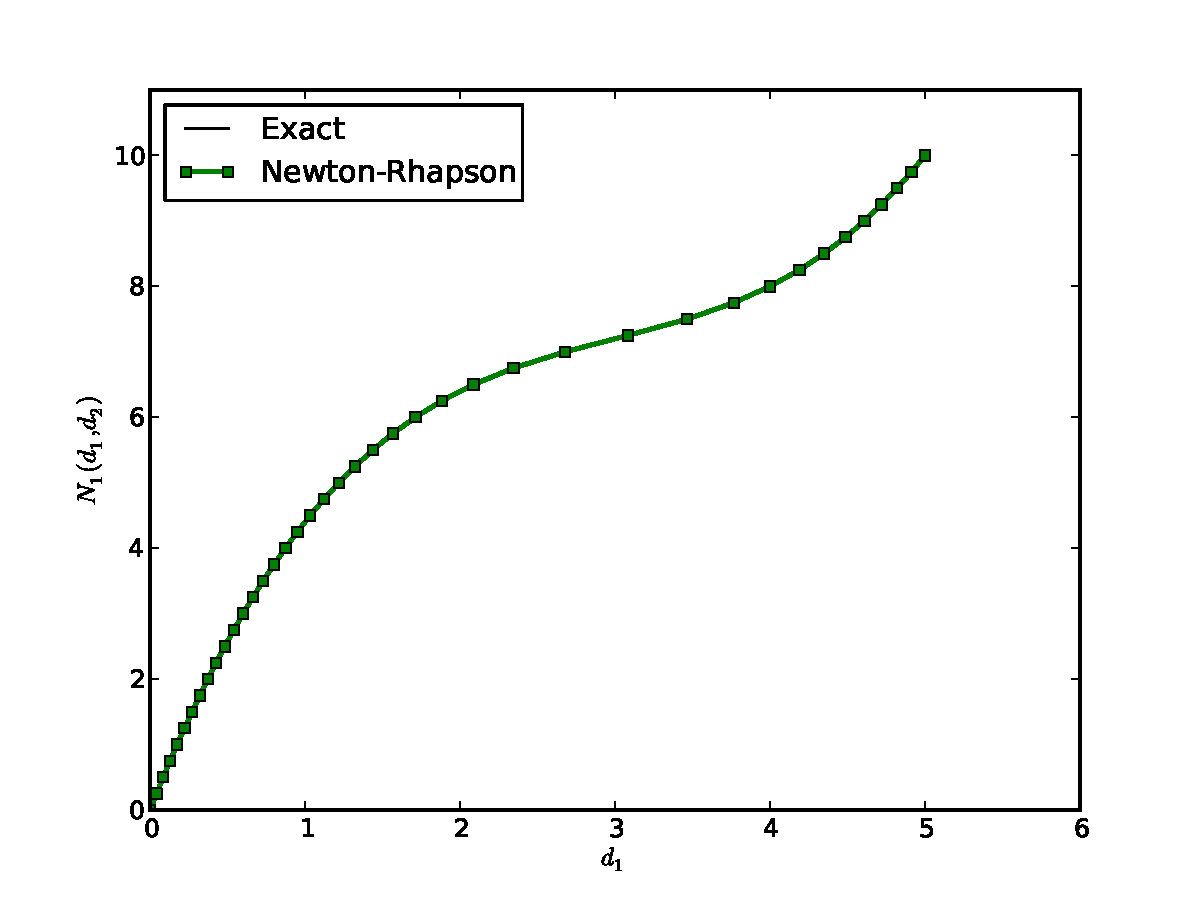
\includegraphics[width=0.75\textwidth]{NR18.pdf}
\caption{Newton-Rhapson, $x=1.8$}
\end{figure}
\begin{figure}[h!]
\centering
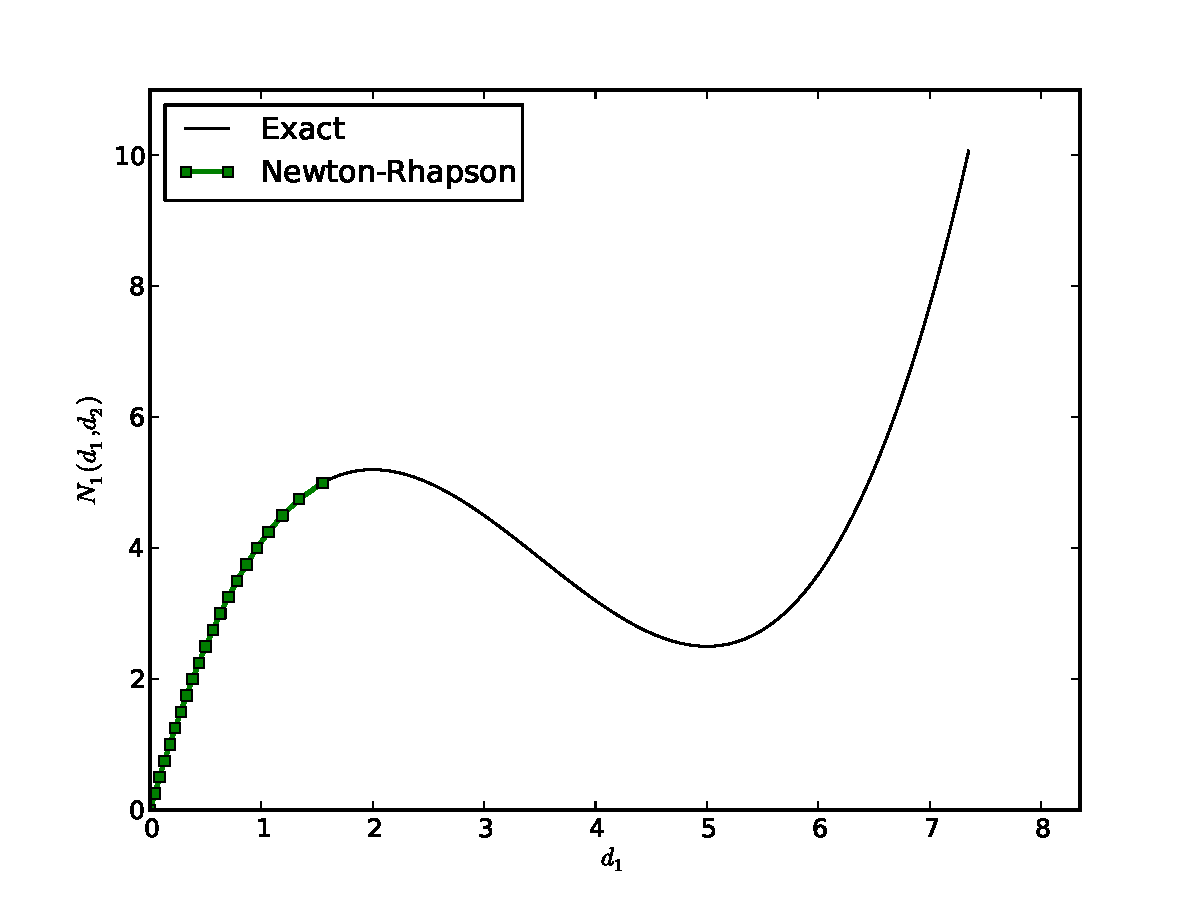
\includegraphics[width=0.75\textwidth]{NR21.pdf}
\caption{Newton-Rhapson, $x=2.1$}
\end{figure}

\begin{figure}[h!]
\centering
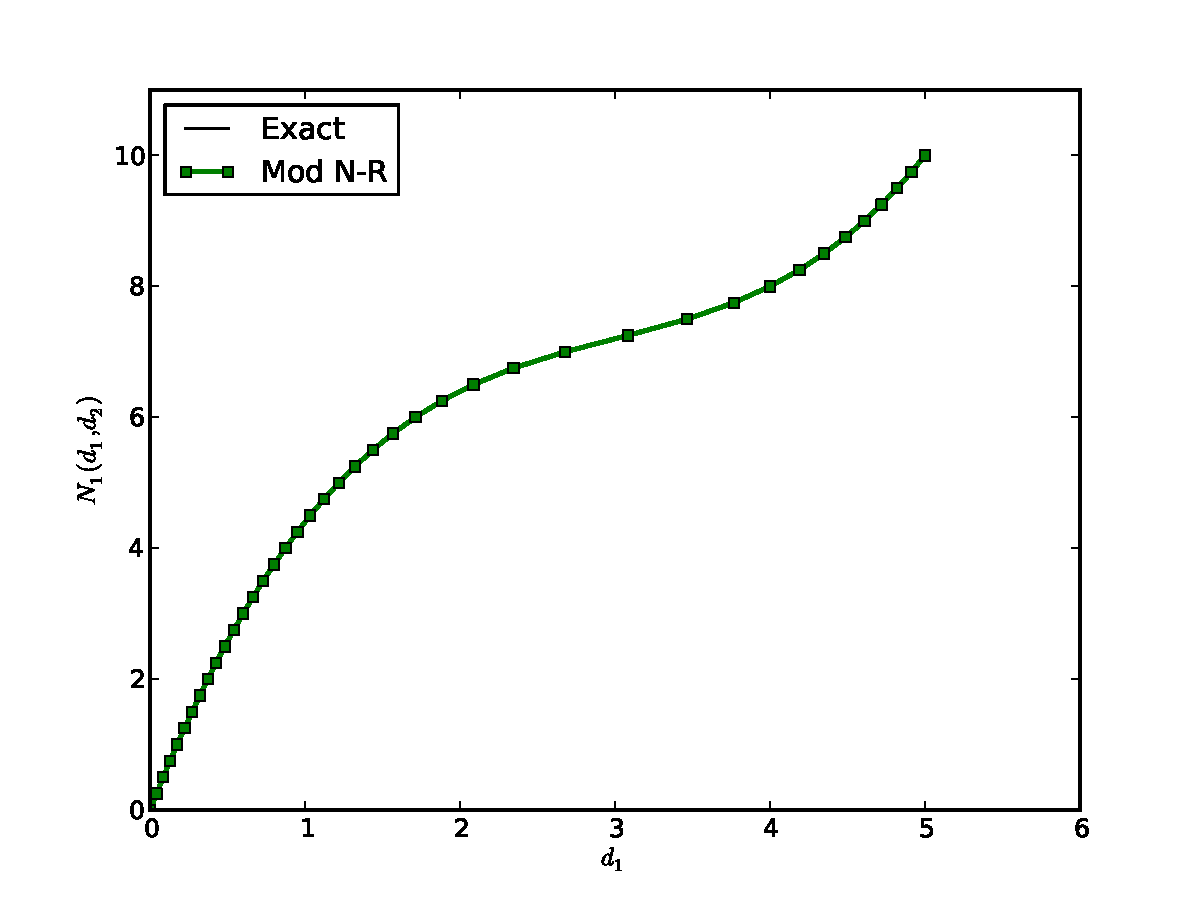
\includegraphics[width=0.75\textwidth]{MNR18.pdf}
\caption{Modified Newton-Rhapson, $x=1.8$}
\end{figure}
\begin{figure}[h!]
\centering
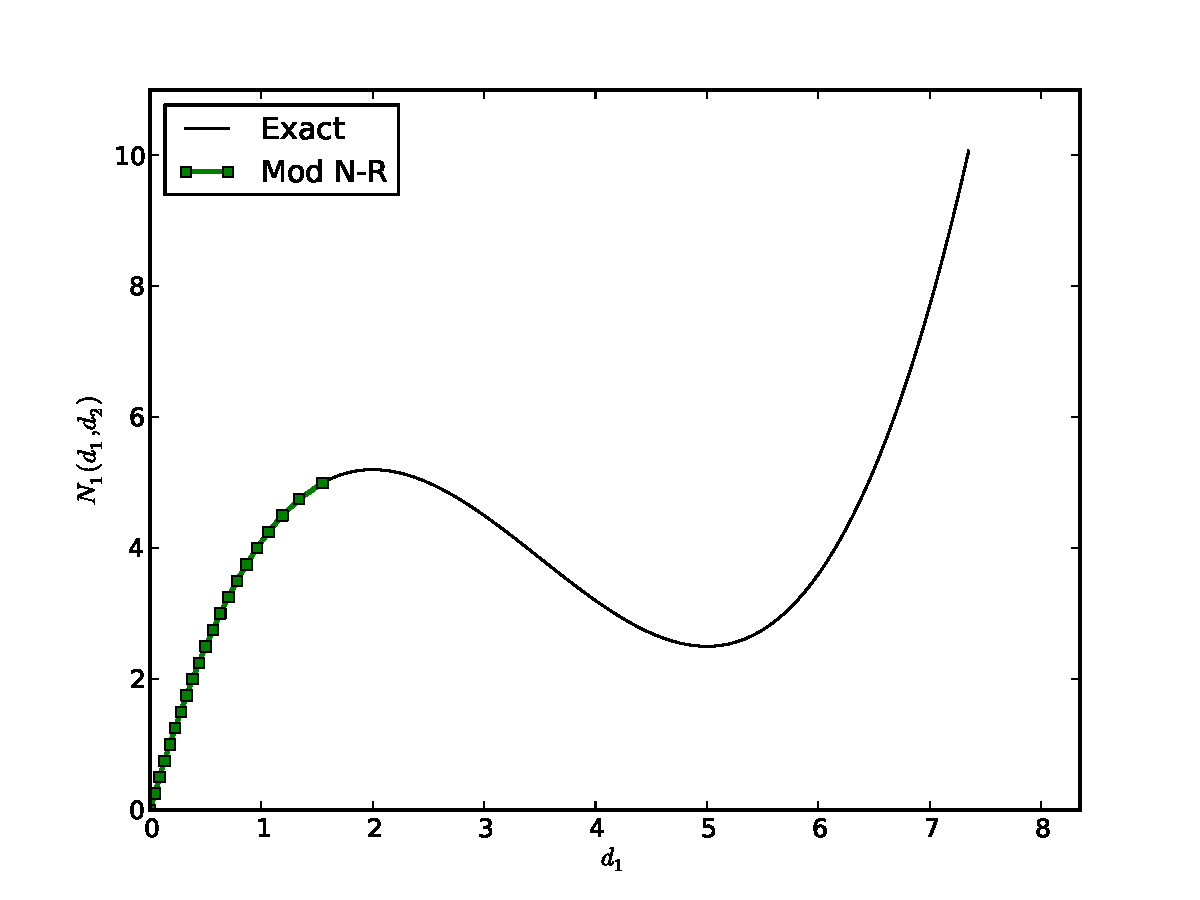
\includegraphics[width=0.75\textwidth]{MNR21.pdf}
\caption{Modified Newton-Rhapson, $x=2.1$}
\end{figure}

\begin{figure}[h!]
\centering
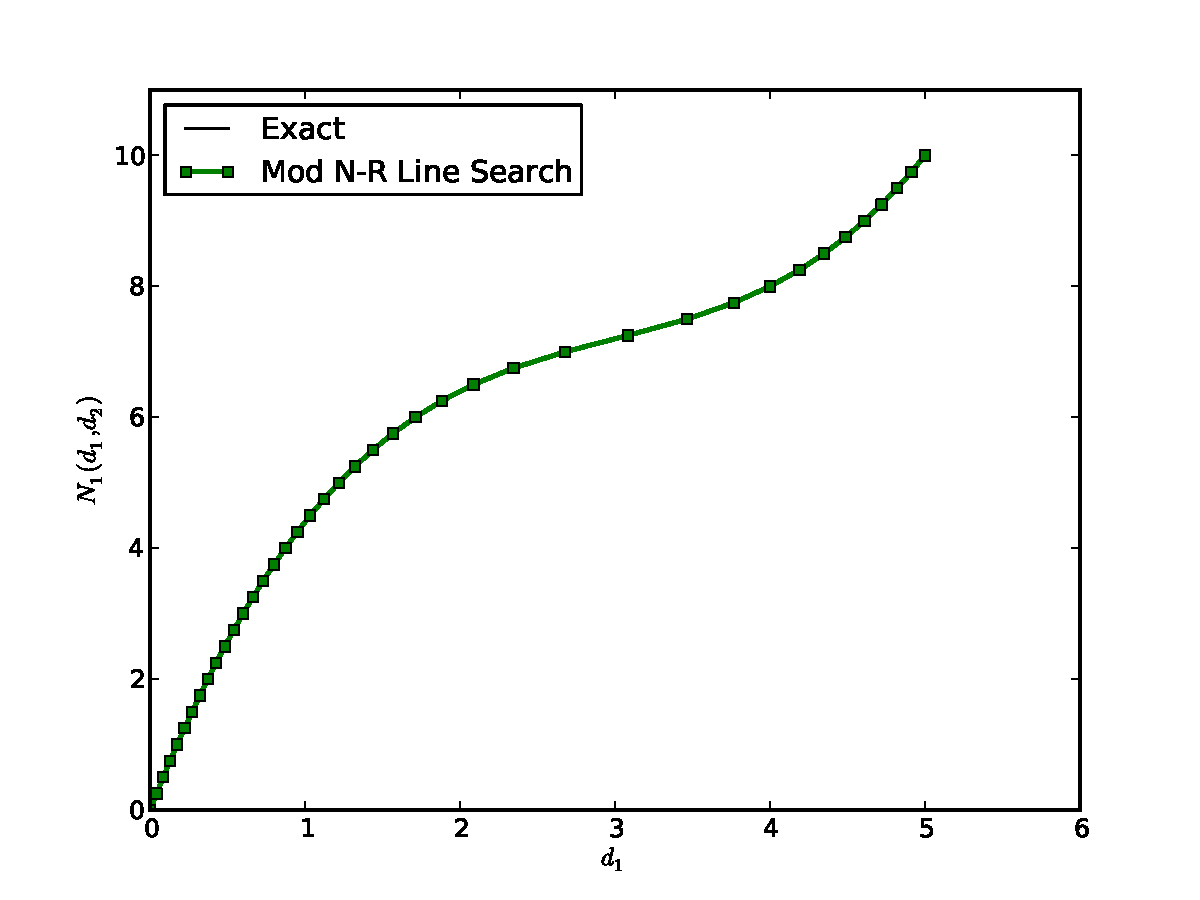
\includegraphics[width=0.75\textwidth]{MNR_LS18.pdf}
\caption{Modified Newton-Rhapson with Line Search, $x=1.8$}
\end{figure}
\begin{figure}[h!]
\centering
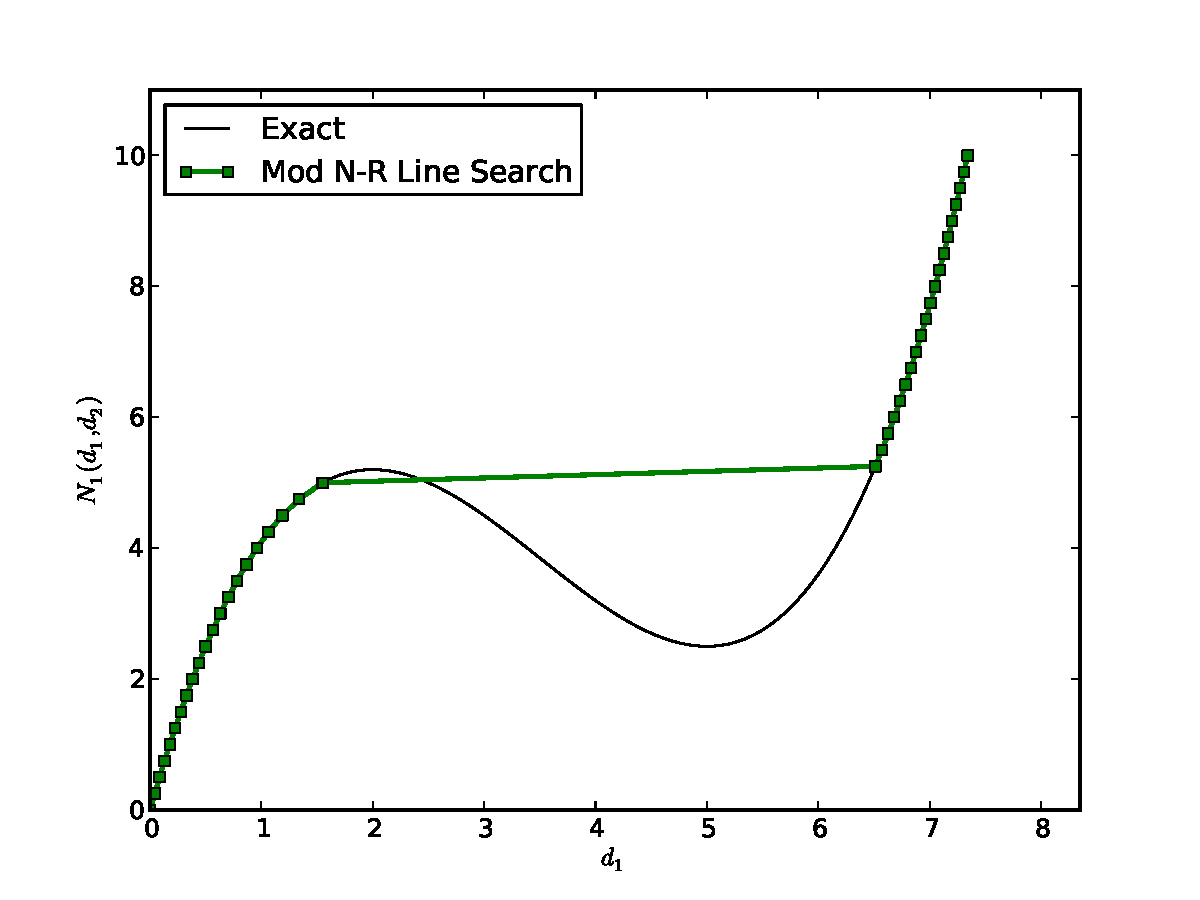
\includegraphics[width=0.75\textwidth]{MNR_LS21.pdf}
\caption{Modified Newton-Rhapson with Line Search, $x=2.1$}
\end{figure}

\begin{figure}[h!]
\centering
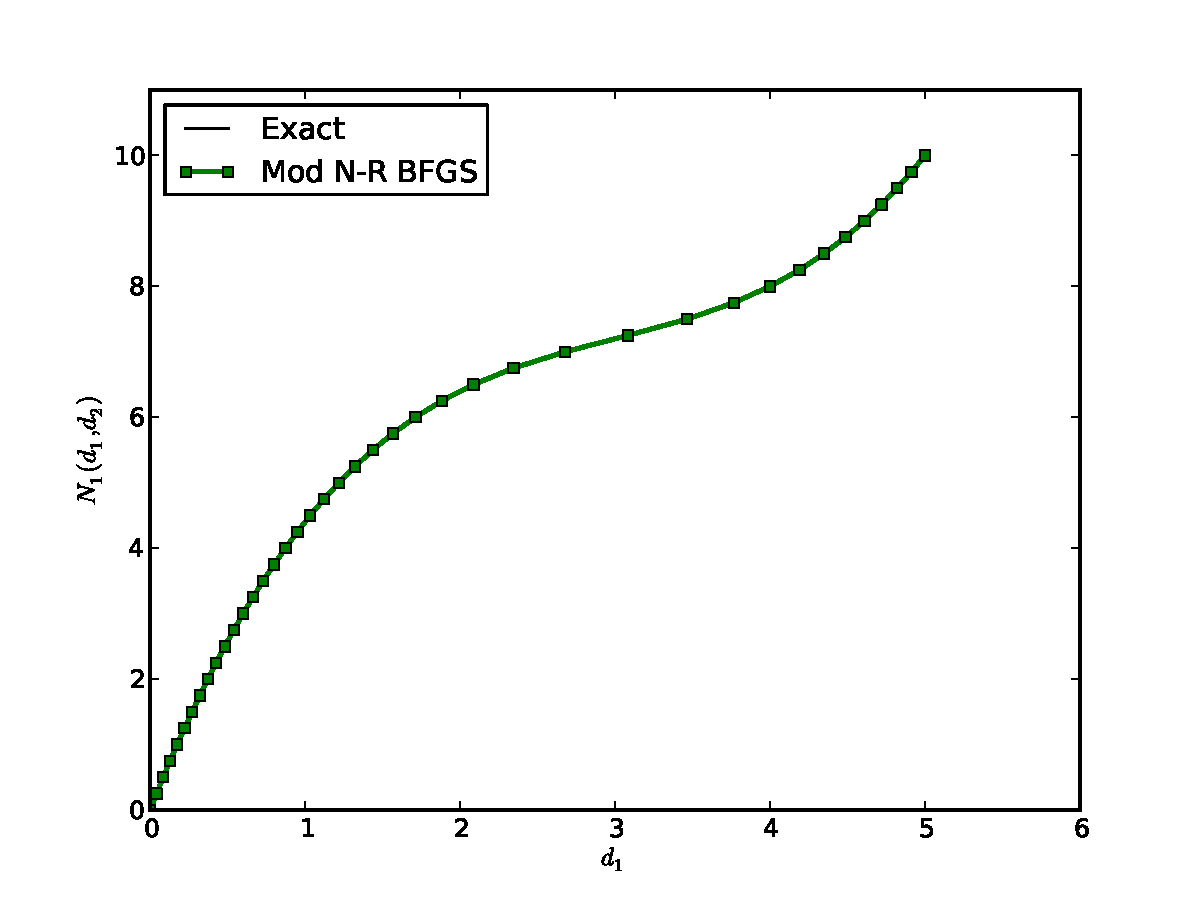
\includegraphics[width=0.75\textwidth]{MNR_BFGS18.pdf}
\caption{Modified Newton-Rhapson with BFGS, $x=1.8$}
\end{figure}
\begin{figure}[h!]
\centering
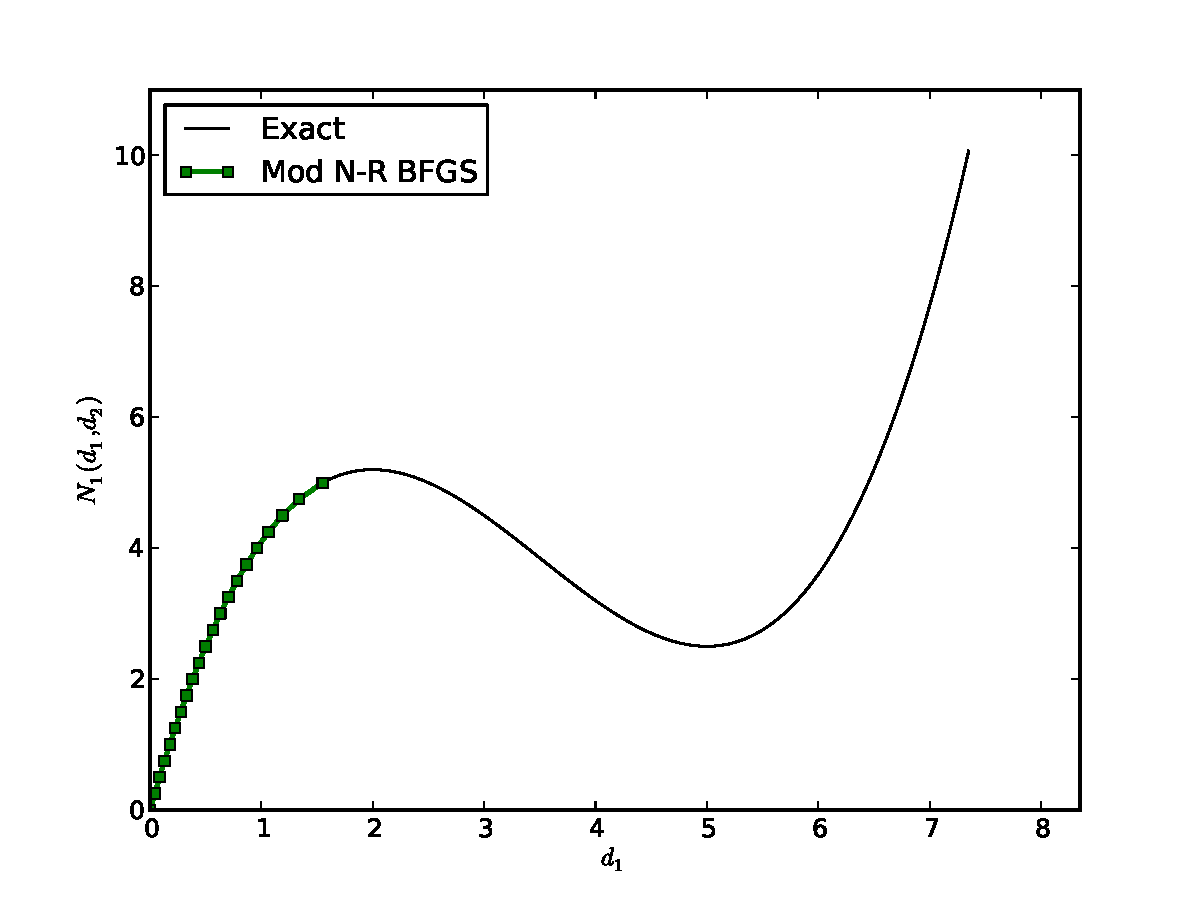
\includegraphics[width=0.75\textwidth]{MNR_BFGS21.pdf}
\caption{Modified Newton-Rhapson with BFGS, $x=2.1$}
\end{figure}

\begin{figure}[h!]
\centering
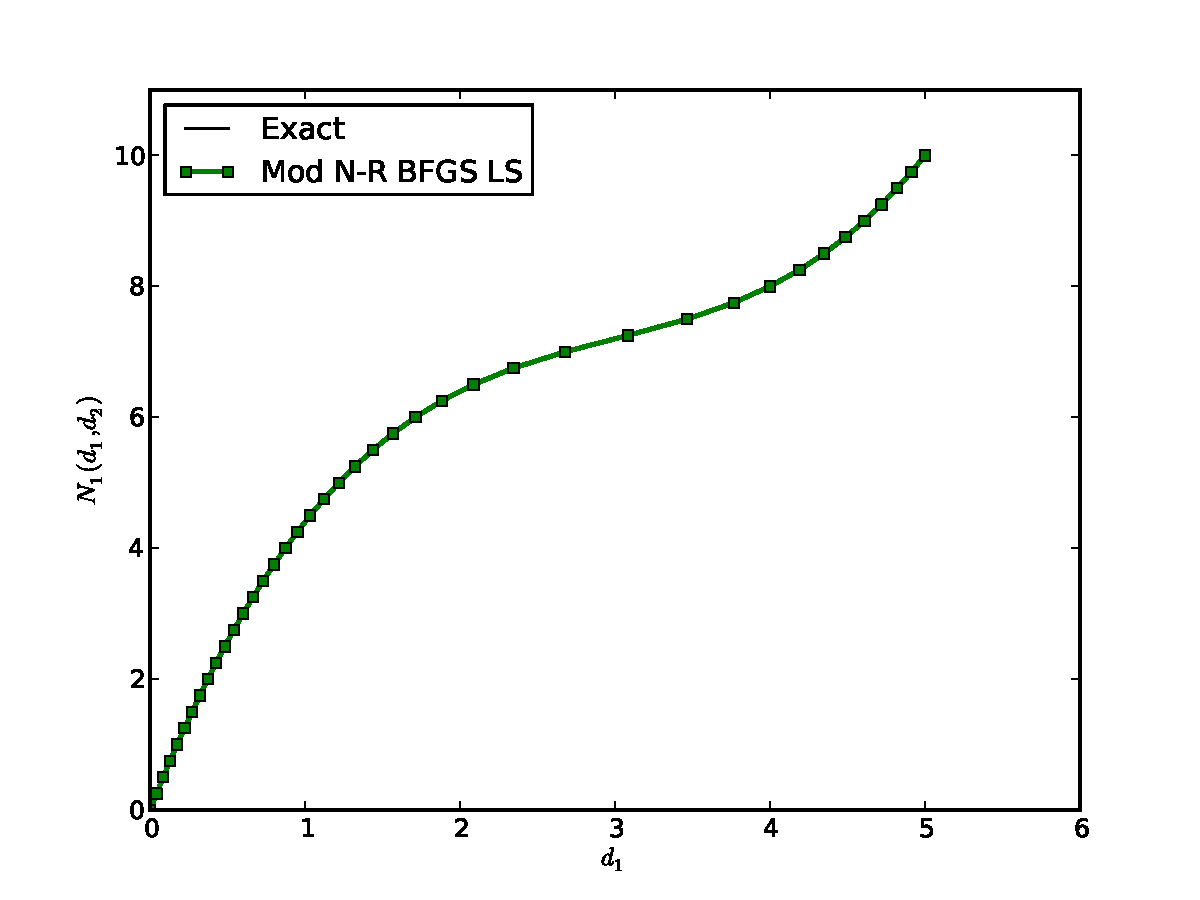
\includegraphics[width=0.75\textwidth]{MNR_BFGS_LS18.pdf}
\caption{Modified Newton-Rhapson with BFGS and Line Search, $x=1.8$}
\end{figure}
\begin{figure}[h!]
\centering
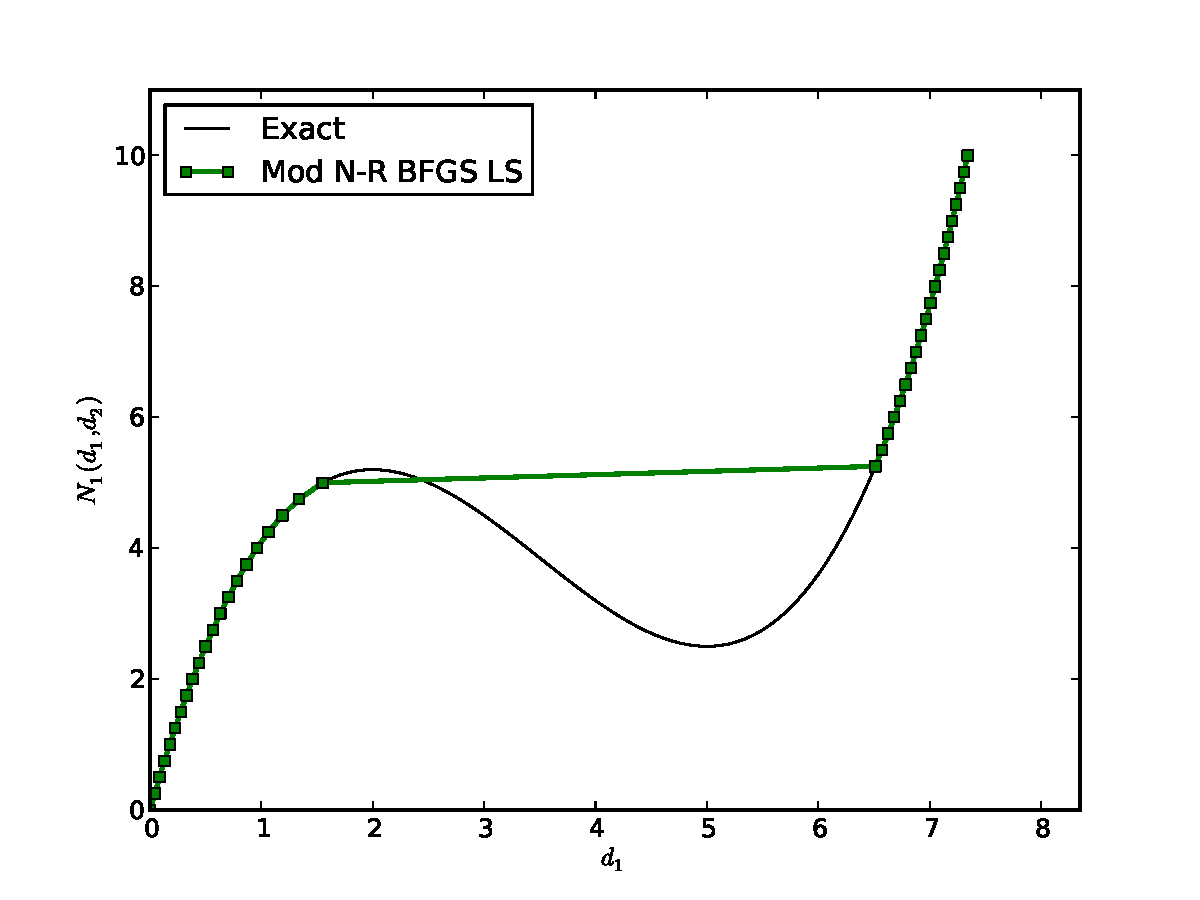
\includegraphics[width=0.75\textwidth]{MNR_BFGS_LS21.pdf}
\caption{Modified Newton-Rhapson with BFGS and Line Search, $x=2.1$}
\end{figure}

\begin{figure}[h!]
\centering
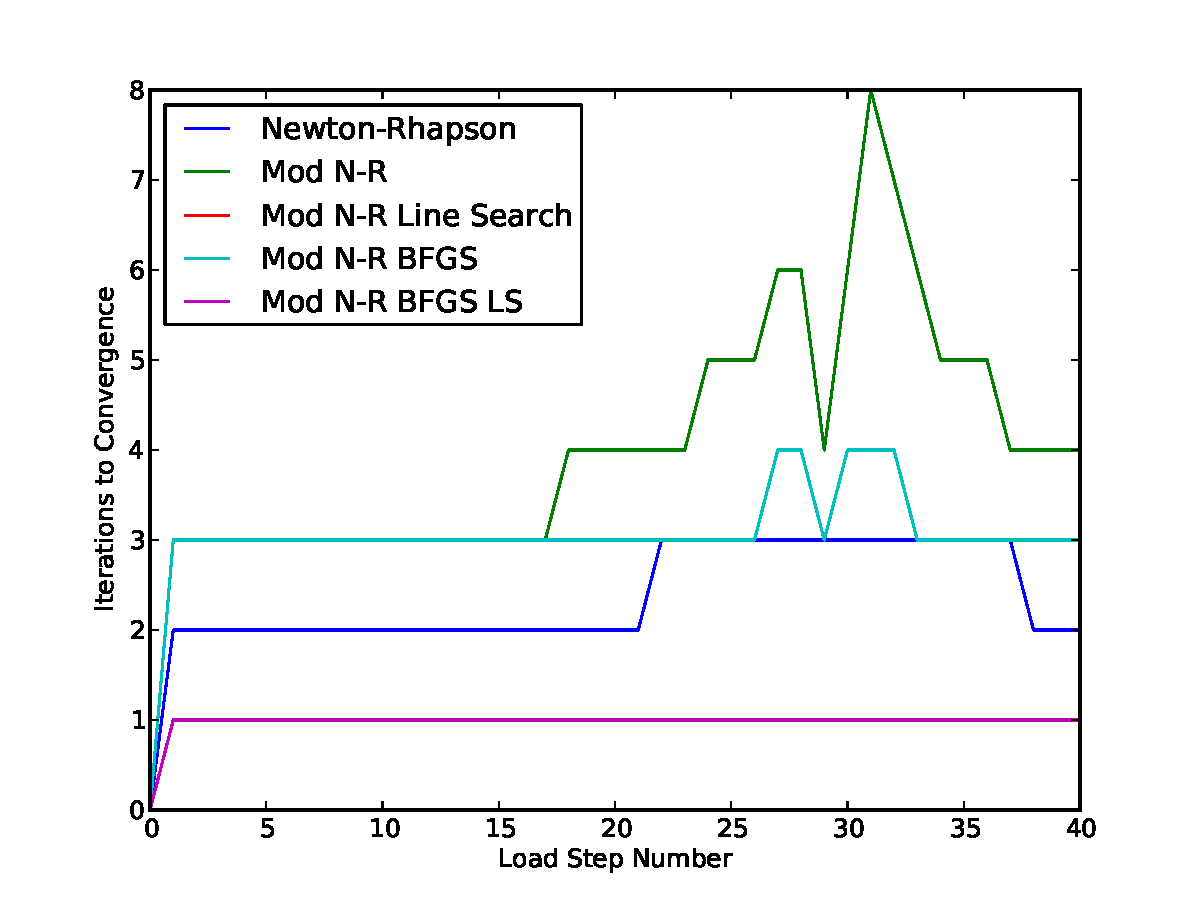
\includegraphics[width=0.75\textwidth]{Iter18.pdf}
\caption{Iterations to convergence, $x=1.8$}
\end{figure}
\begin{figure}[h!]
\centering
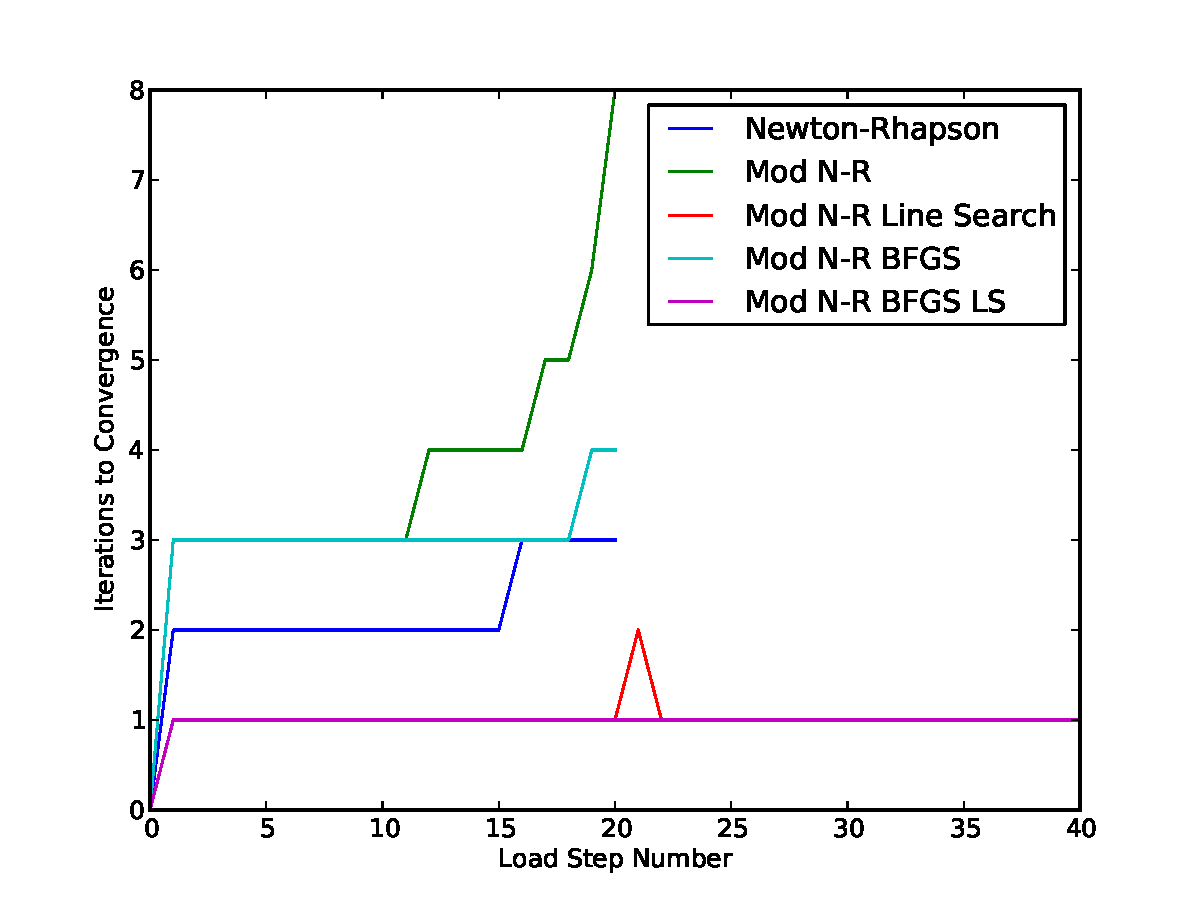
\includegraphics[width=0.75\textwidth]{Iter21.pdf}
\caption{Iterations to convergence, $x=2.1$}
\end{figure}

\clearpage
\newpage
\lstinputlisting[language=Python,title={Homework5.py}]{HW5.py}

\end{document}
